\documentclass{beamer}
\usetheme{Berlin}
\usecolortheme{dolphin}

\usepackage[T1]{polski}
\usepackage[polish]{babel}
\usepackage[utf8]{inputenc}
\usepackage[T1]{fontenc}
\usepackage[mediumspace,mediumqspace,Grey,squaren]{SIunits}
\usepackage{graphicx}
\usepackage{hyperref}

%\addbibresource{bibliography.bib}

%\setbeamertemplate{bibliography item}{\insertbiblabel}


\graphicspath{ {./images/} }

\begin{document}
\title{Seminarium dyplomowe magisterskie}
\author{Jakub Postępski}
\date{29 listopada 2018}

\frame{\titlepage}

\section{Zarys pracy magisterskiej}

\begin{frame}{Sterowanie ramieniem robota w obliczu chwytania przedmiotów}

Kompensacja siły grawitacji (i~sił pozornych) działających na przedmiot chwycony przez robota sterowanego siłowo.

\begin{itemize}
	\item Dr inż. Tomasz Winiarski.
	\item Laboratorium robotyki.
\end{itemize}

\begin{itemize}
	\item Podnoszenie obiektu bez identyfikacji.
	\item Identyfikacja.
	\item Manipulacja zidentyfikowanym obiektem.
	\item Manipulacja i identyfikacja w jednym.
\end{itemize}
\end{frame}

\begin{frame}{Rozgrzewka}
\begin{figure}[h]
	\centering
	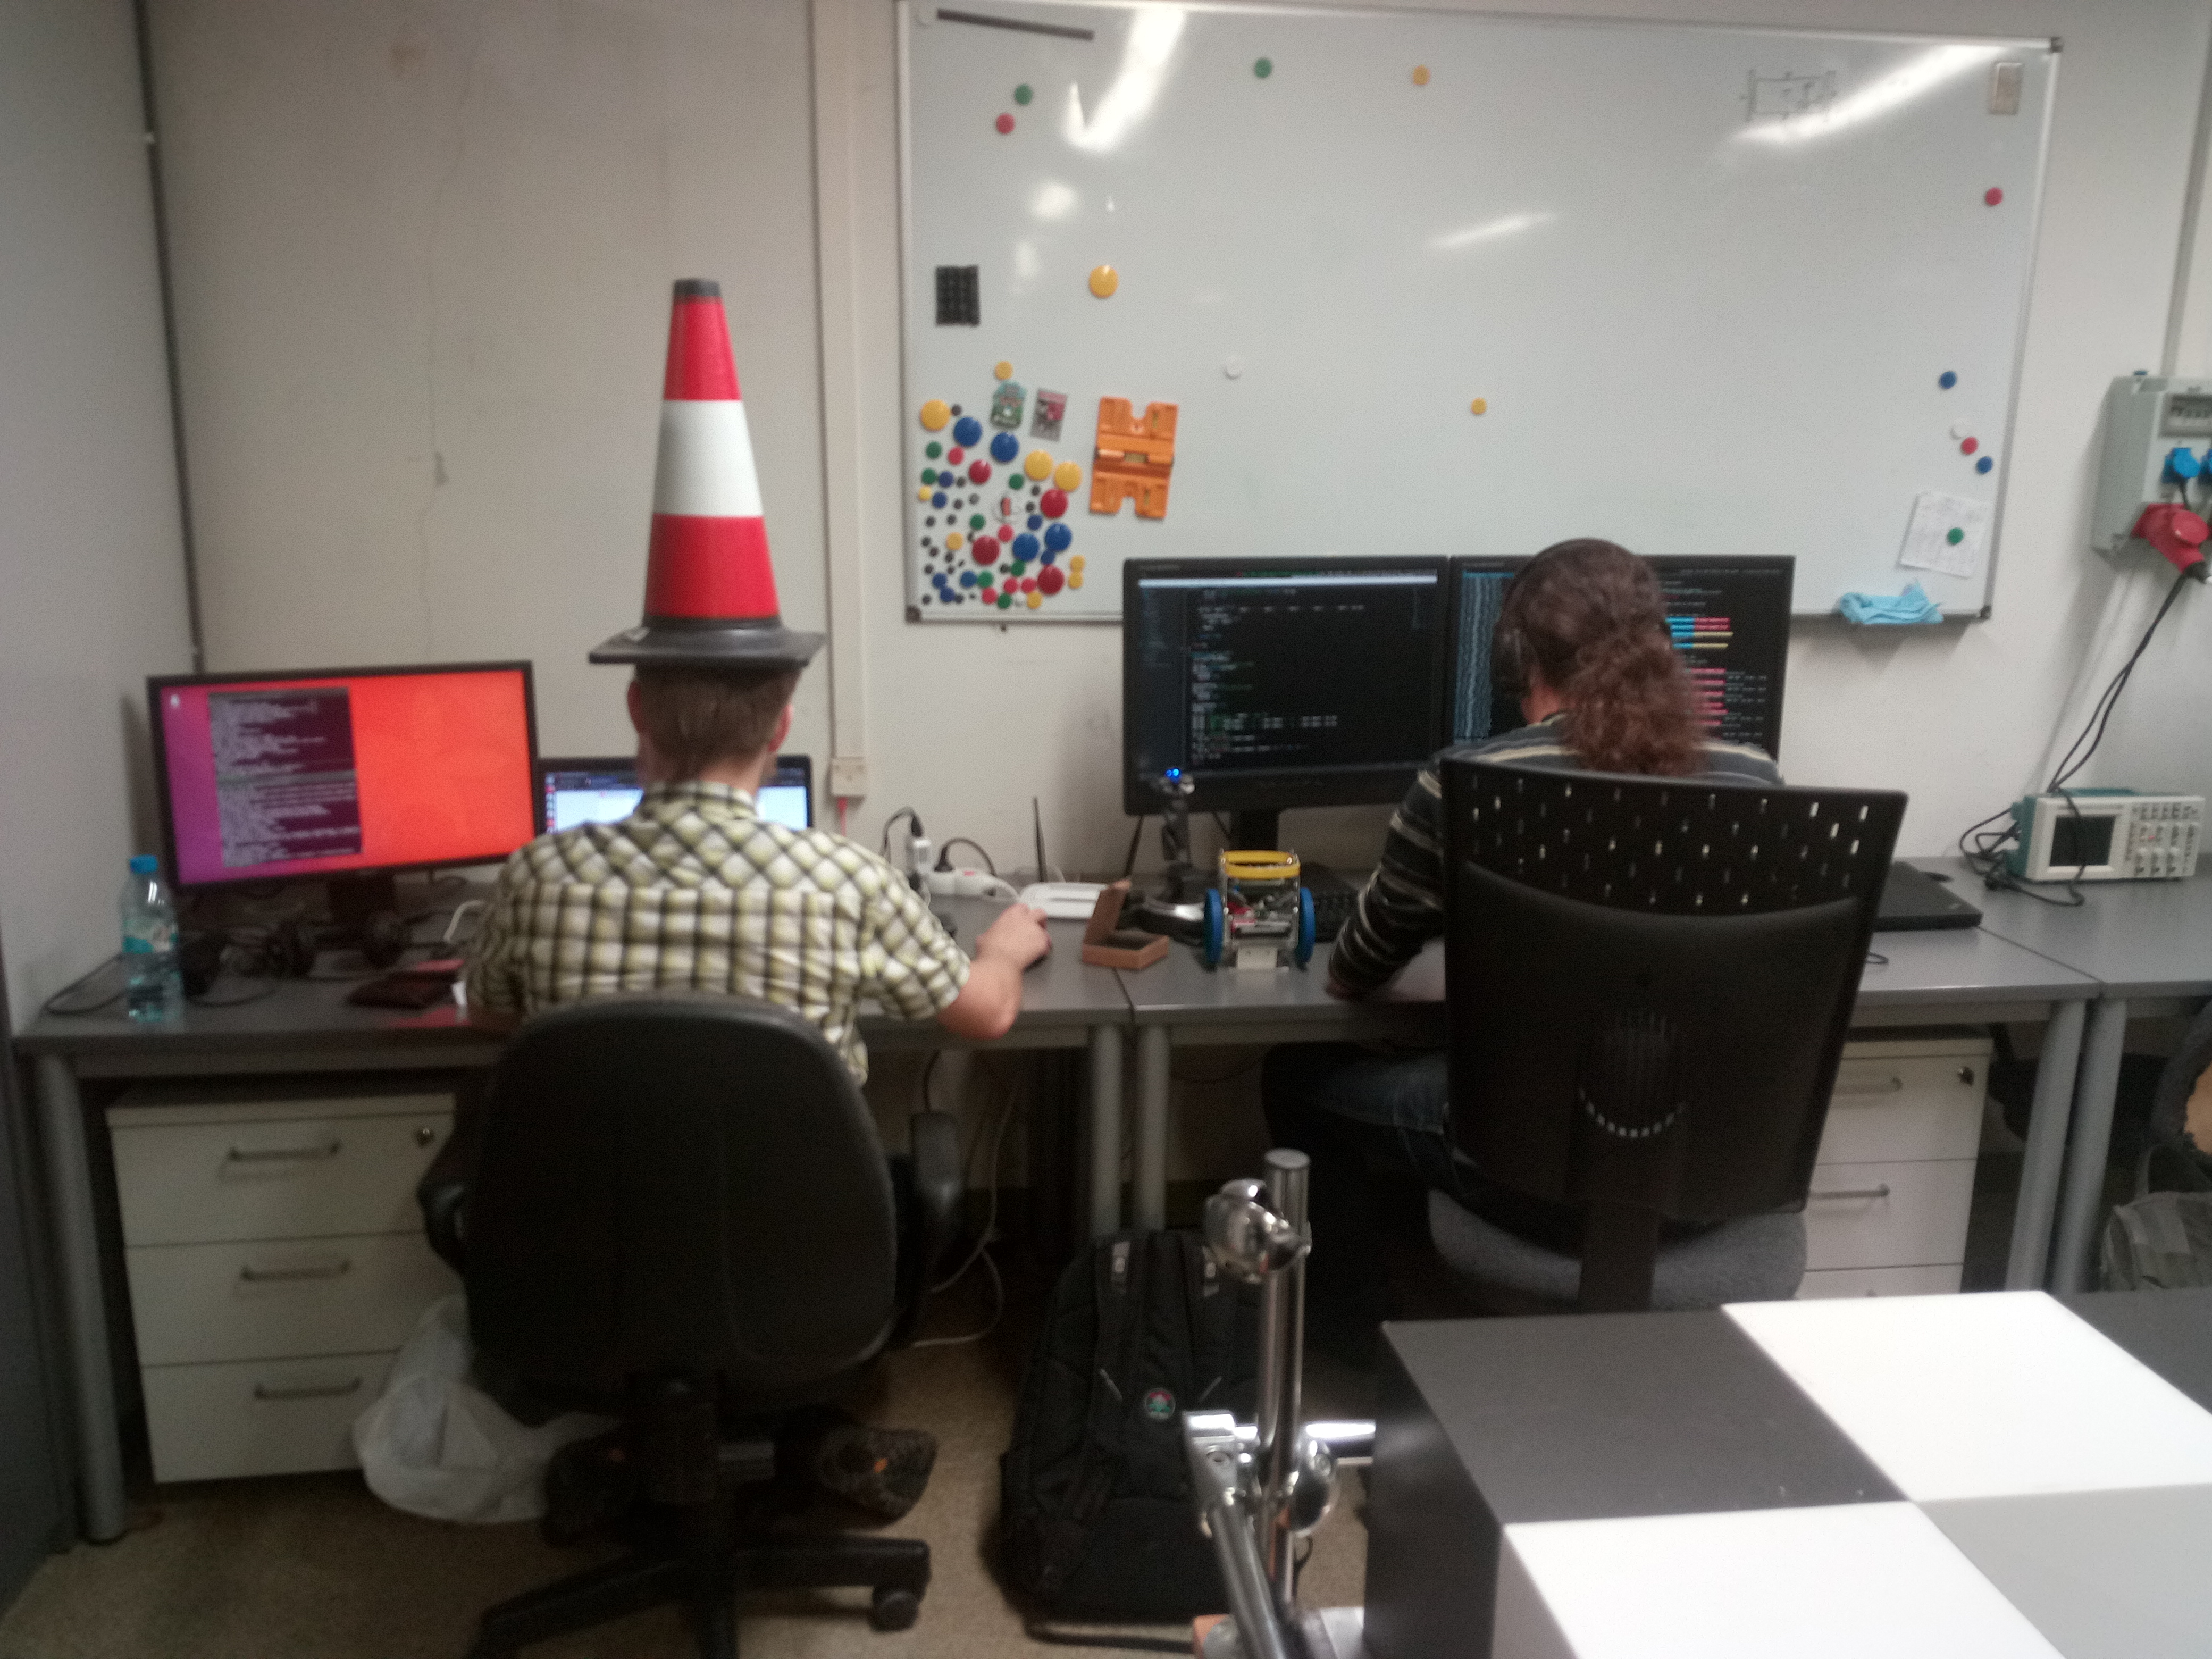
\includegraphics[scale=0.06]{daniel}
\end{figure}
\end{frame}

\begin{frame}{Sterowanie impedancyjne}
\[ m\ddot{x} + b\dot{x} + kx = f_{ext} \]
\begin{figure}
	\centering
	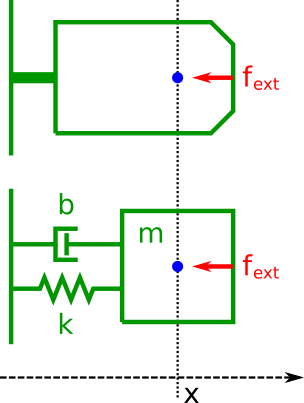
\includegraphics[scale=1]{impedance}
\end{figure}
\end{frame}

\begin{frame}{Założenia i ograniczenia}
\begin{itemize}
	\item Sterowanie impedancyjne.
	\item Nieznany model chwytanego obiektu.
	\item Obiekt chwytany przez robota może zmieniać się w czasie.
	\item Założenia modelu jak dla bryły sztywnej.
	\item Możliwe, że badania zakończą się tylko na przypadkach statycznych.
	\item Brak masy ramienia robota.
\end{itemize}
\end{frame}

\section{Środowisko badawcze}

\begin{frame}{Robot usługowy Velma}
\begin{itemize}
\item Dwa manipulatory LWR
\item Chwytaki Barretta (sztuczna skóra, czujniki siły)
\item Nadgarstkowe FTS
\item Kinect
\item Stereopara
\item Komputer sterujący
\end{itemize}
\end{frame}

\begin{frame}{Zdjęcie robota Velma}
	\begin{figure}[h]
		\centering
		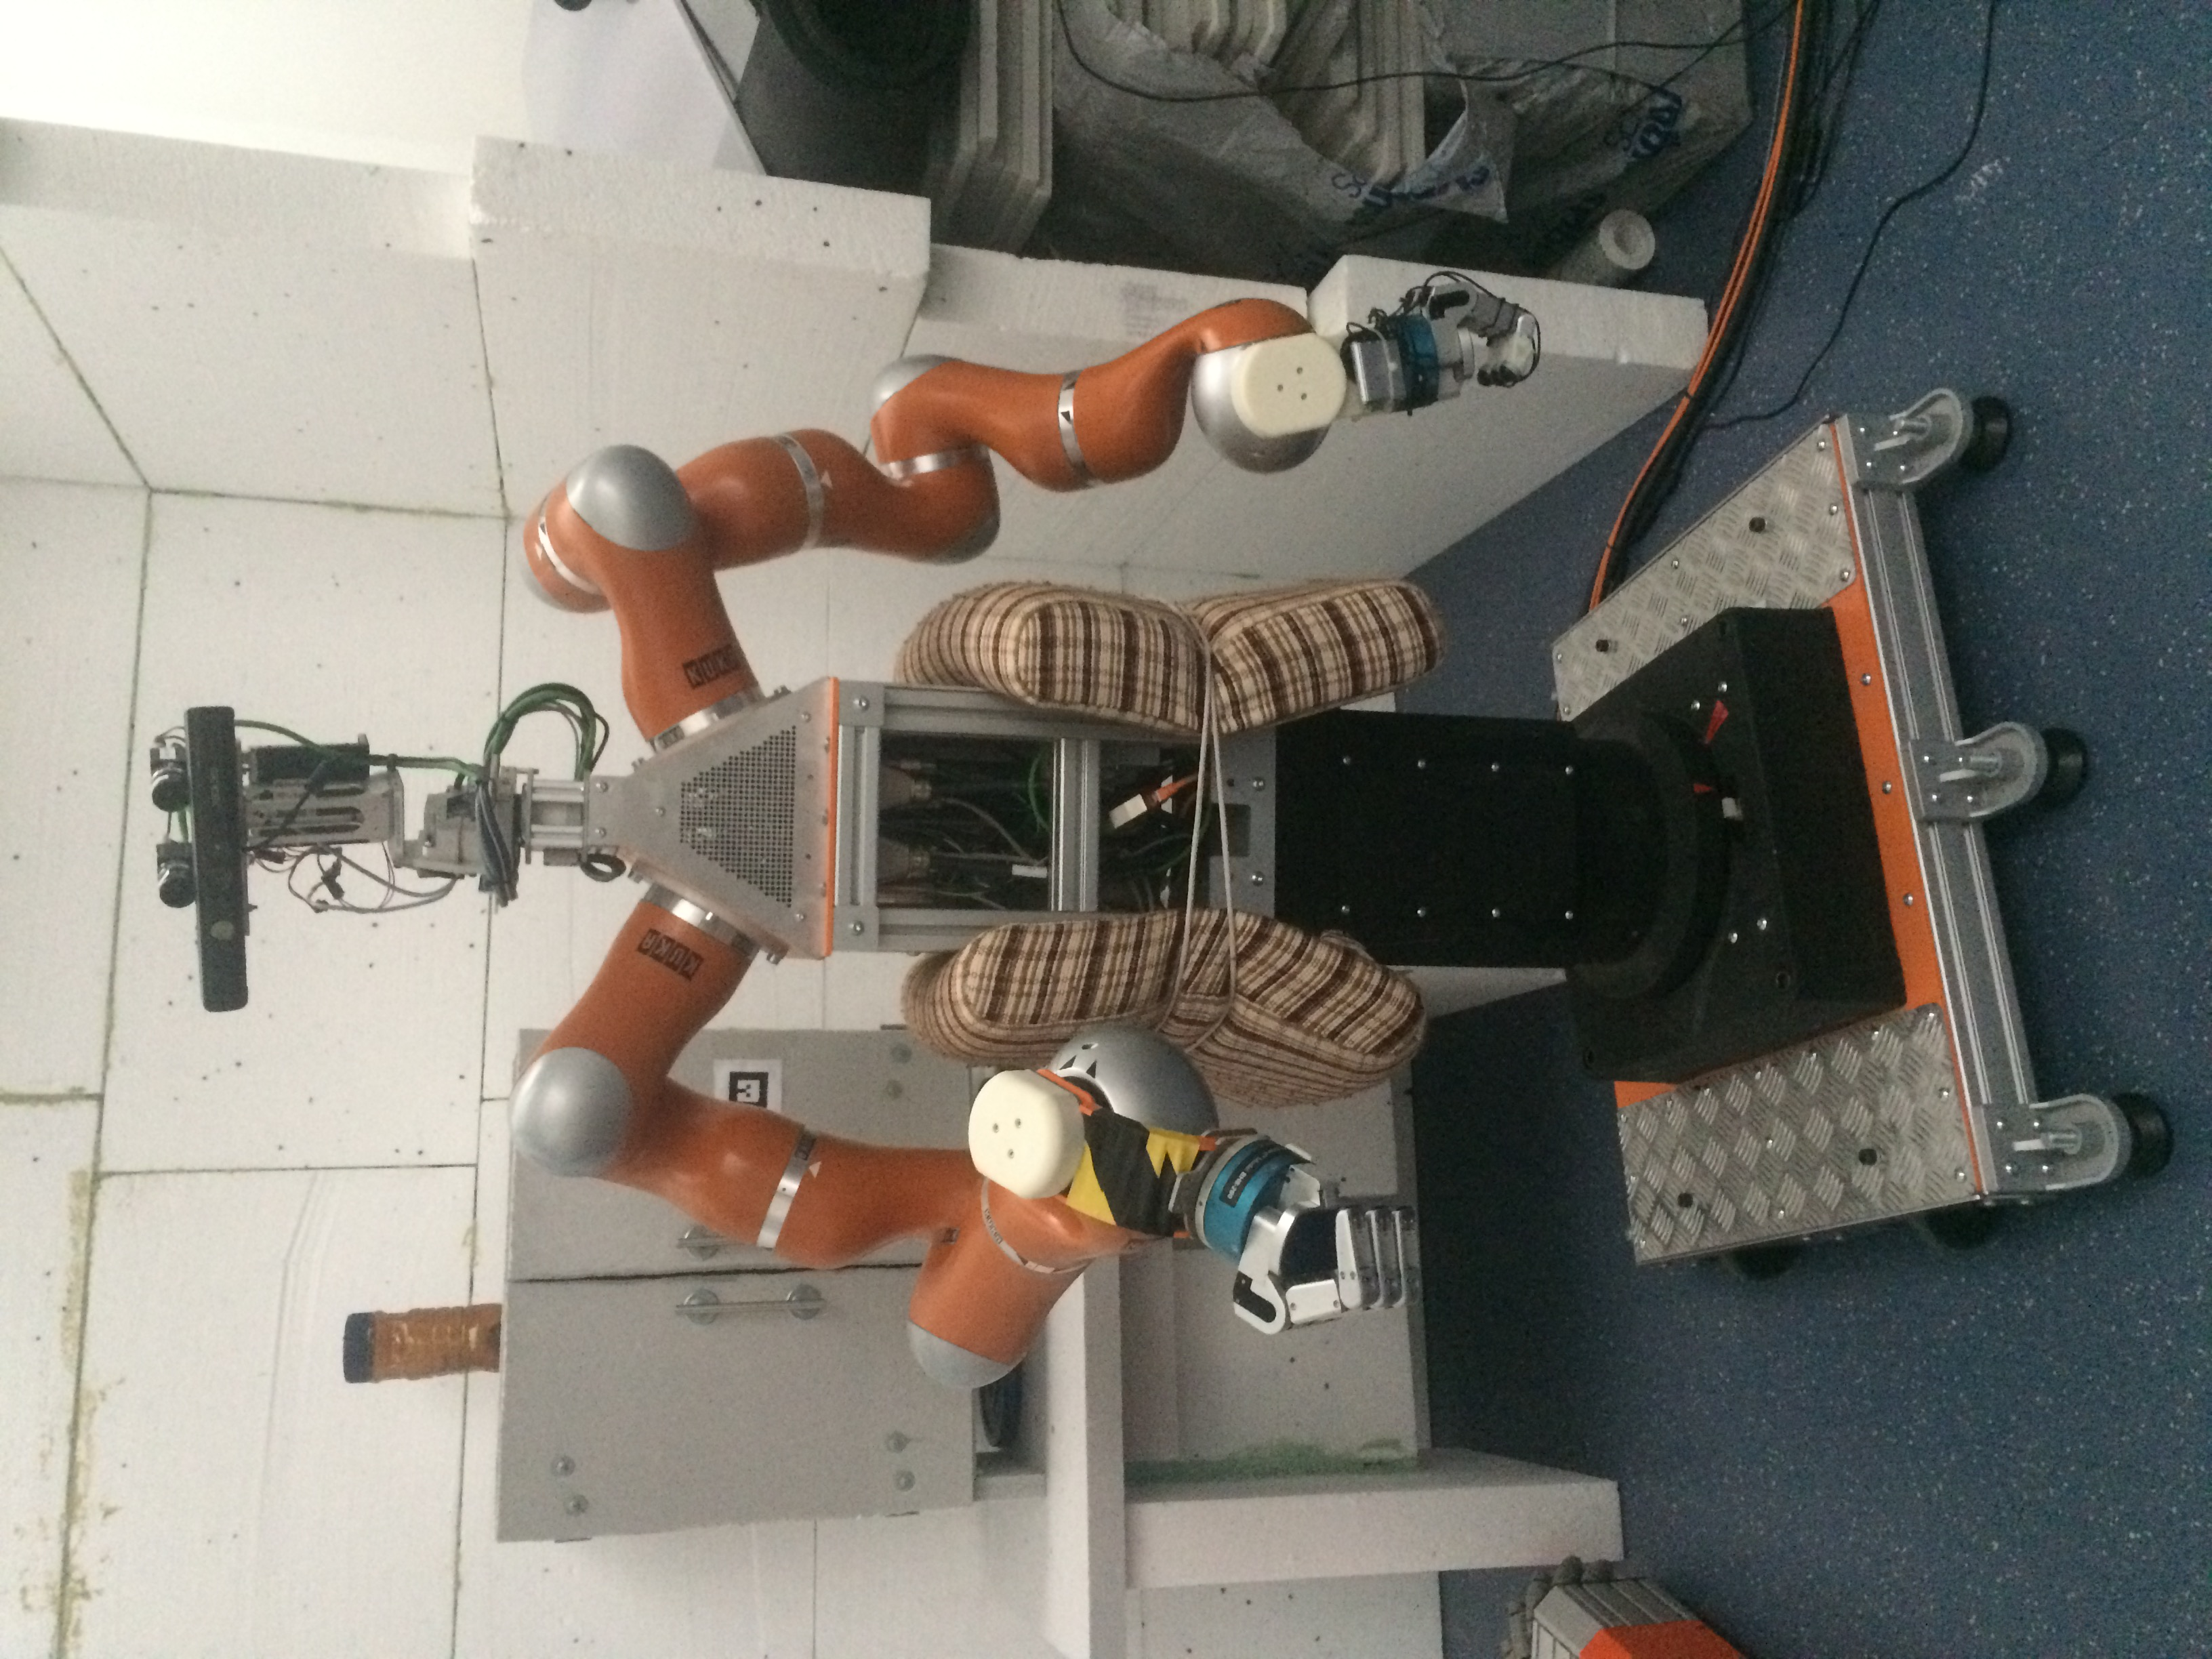
\includegraphics[scale=0.055, angle =-90]{velma1}
	\end{figure}
\end{frame}

\begin{frame}{Kuka LWR}
\begin{figure}[h]
	\centering
	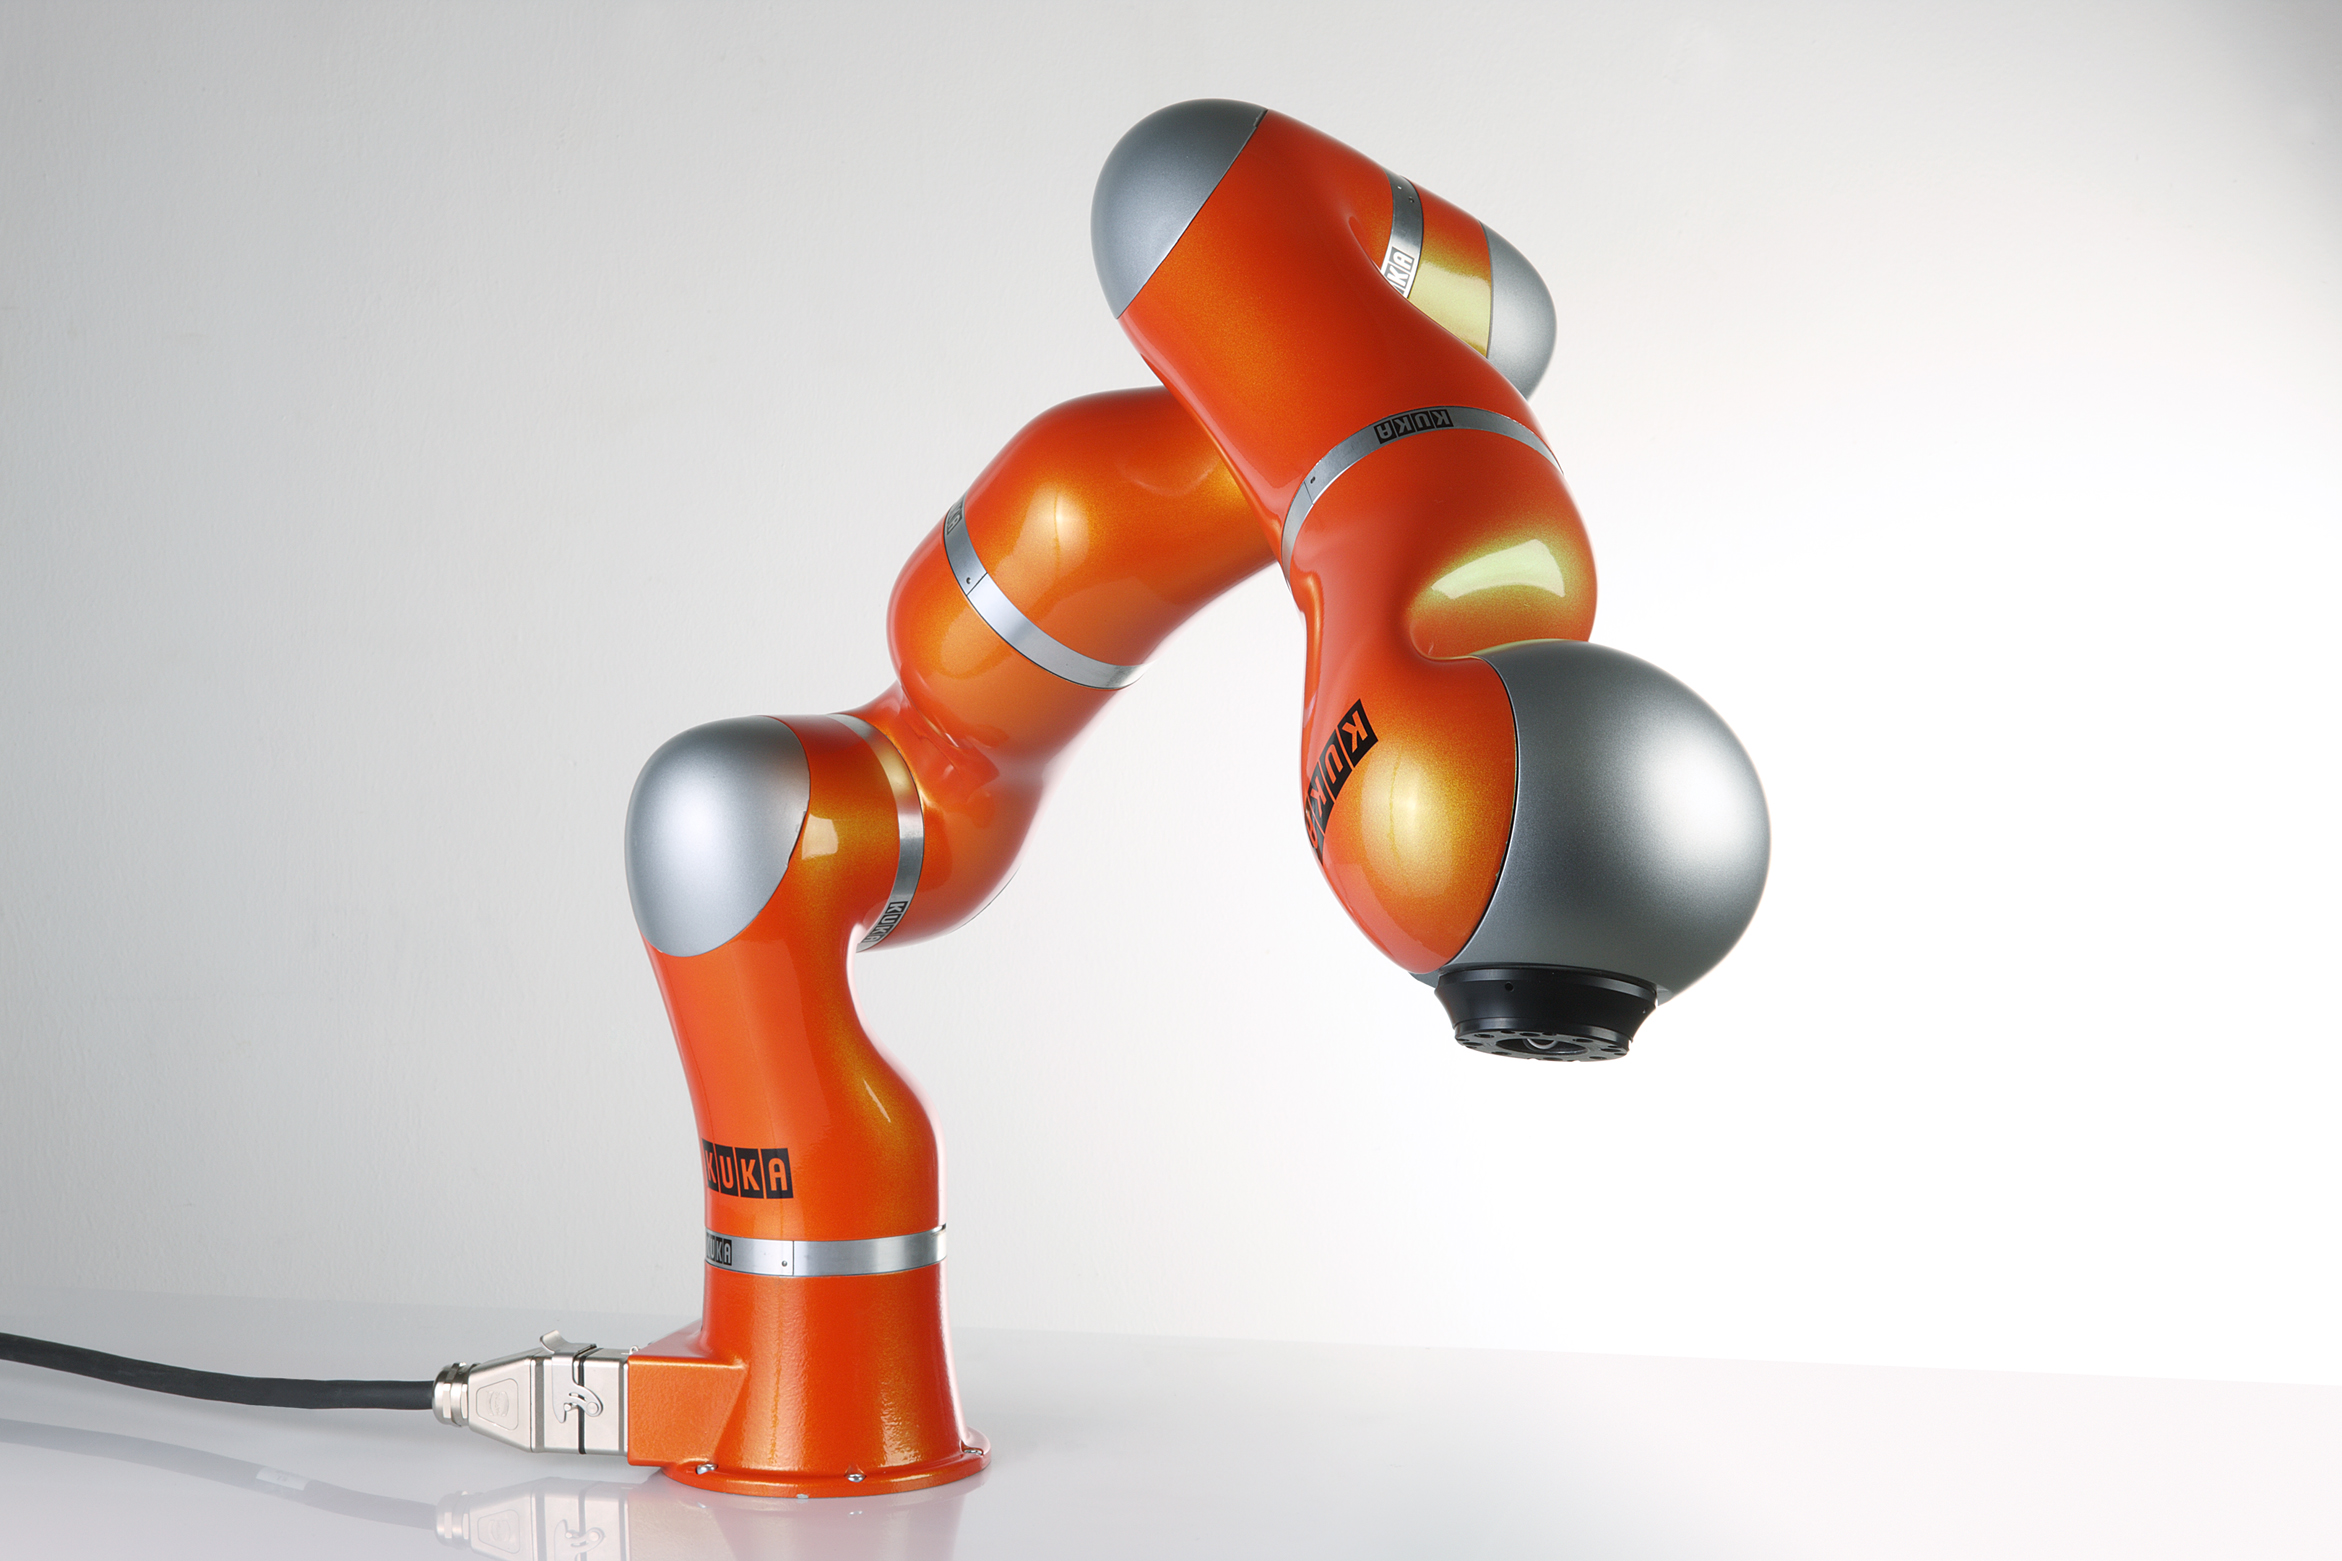
\includegraphics[scale=0.5]{kuka}
\end{figure}
\end{frame}

\begin{frame}{FTS}
\begin{figure}[h]
	\centering
	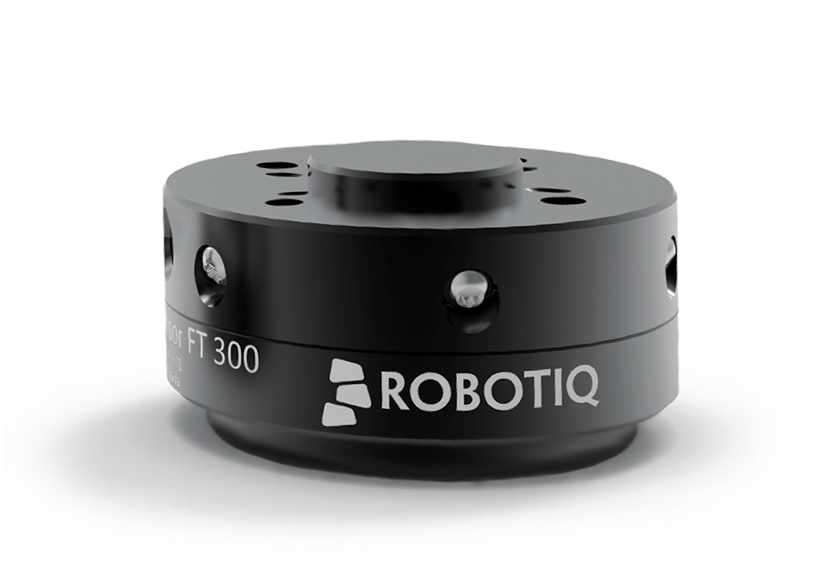
\includegraphics[scale=0.35]{fts}
\end{figure}
\end{frame}

\begin{frame}{Chwytak Barretta}
\begin{figure}[h]
	\centering
	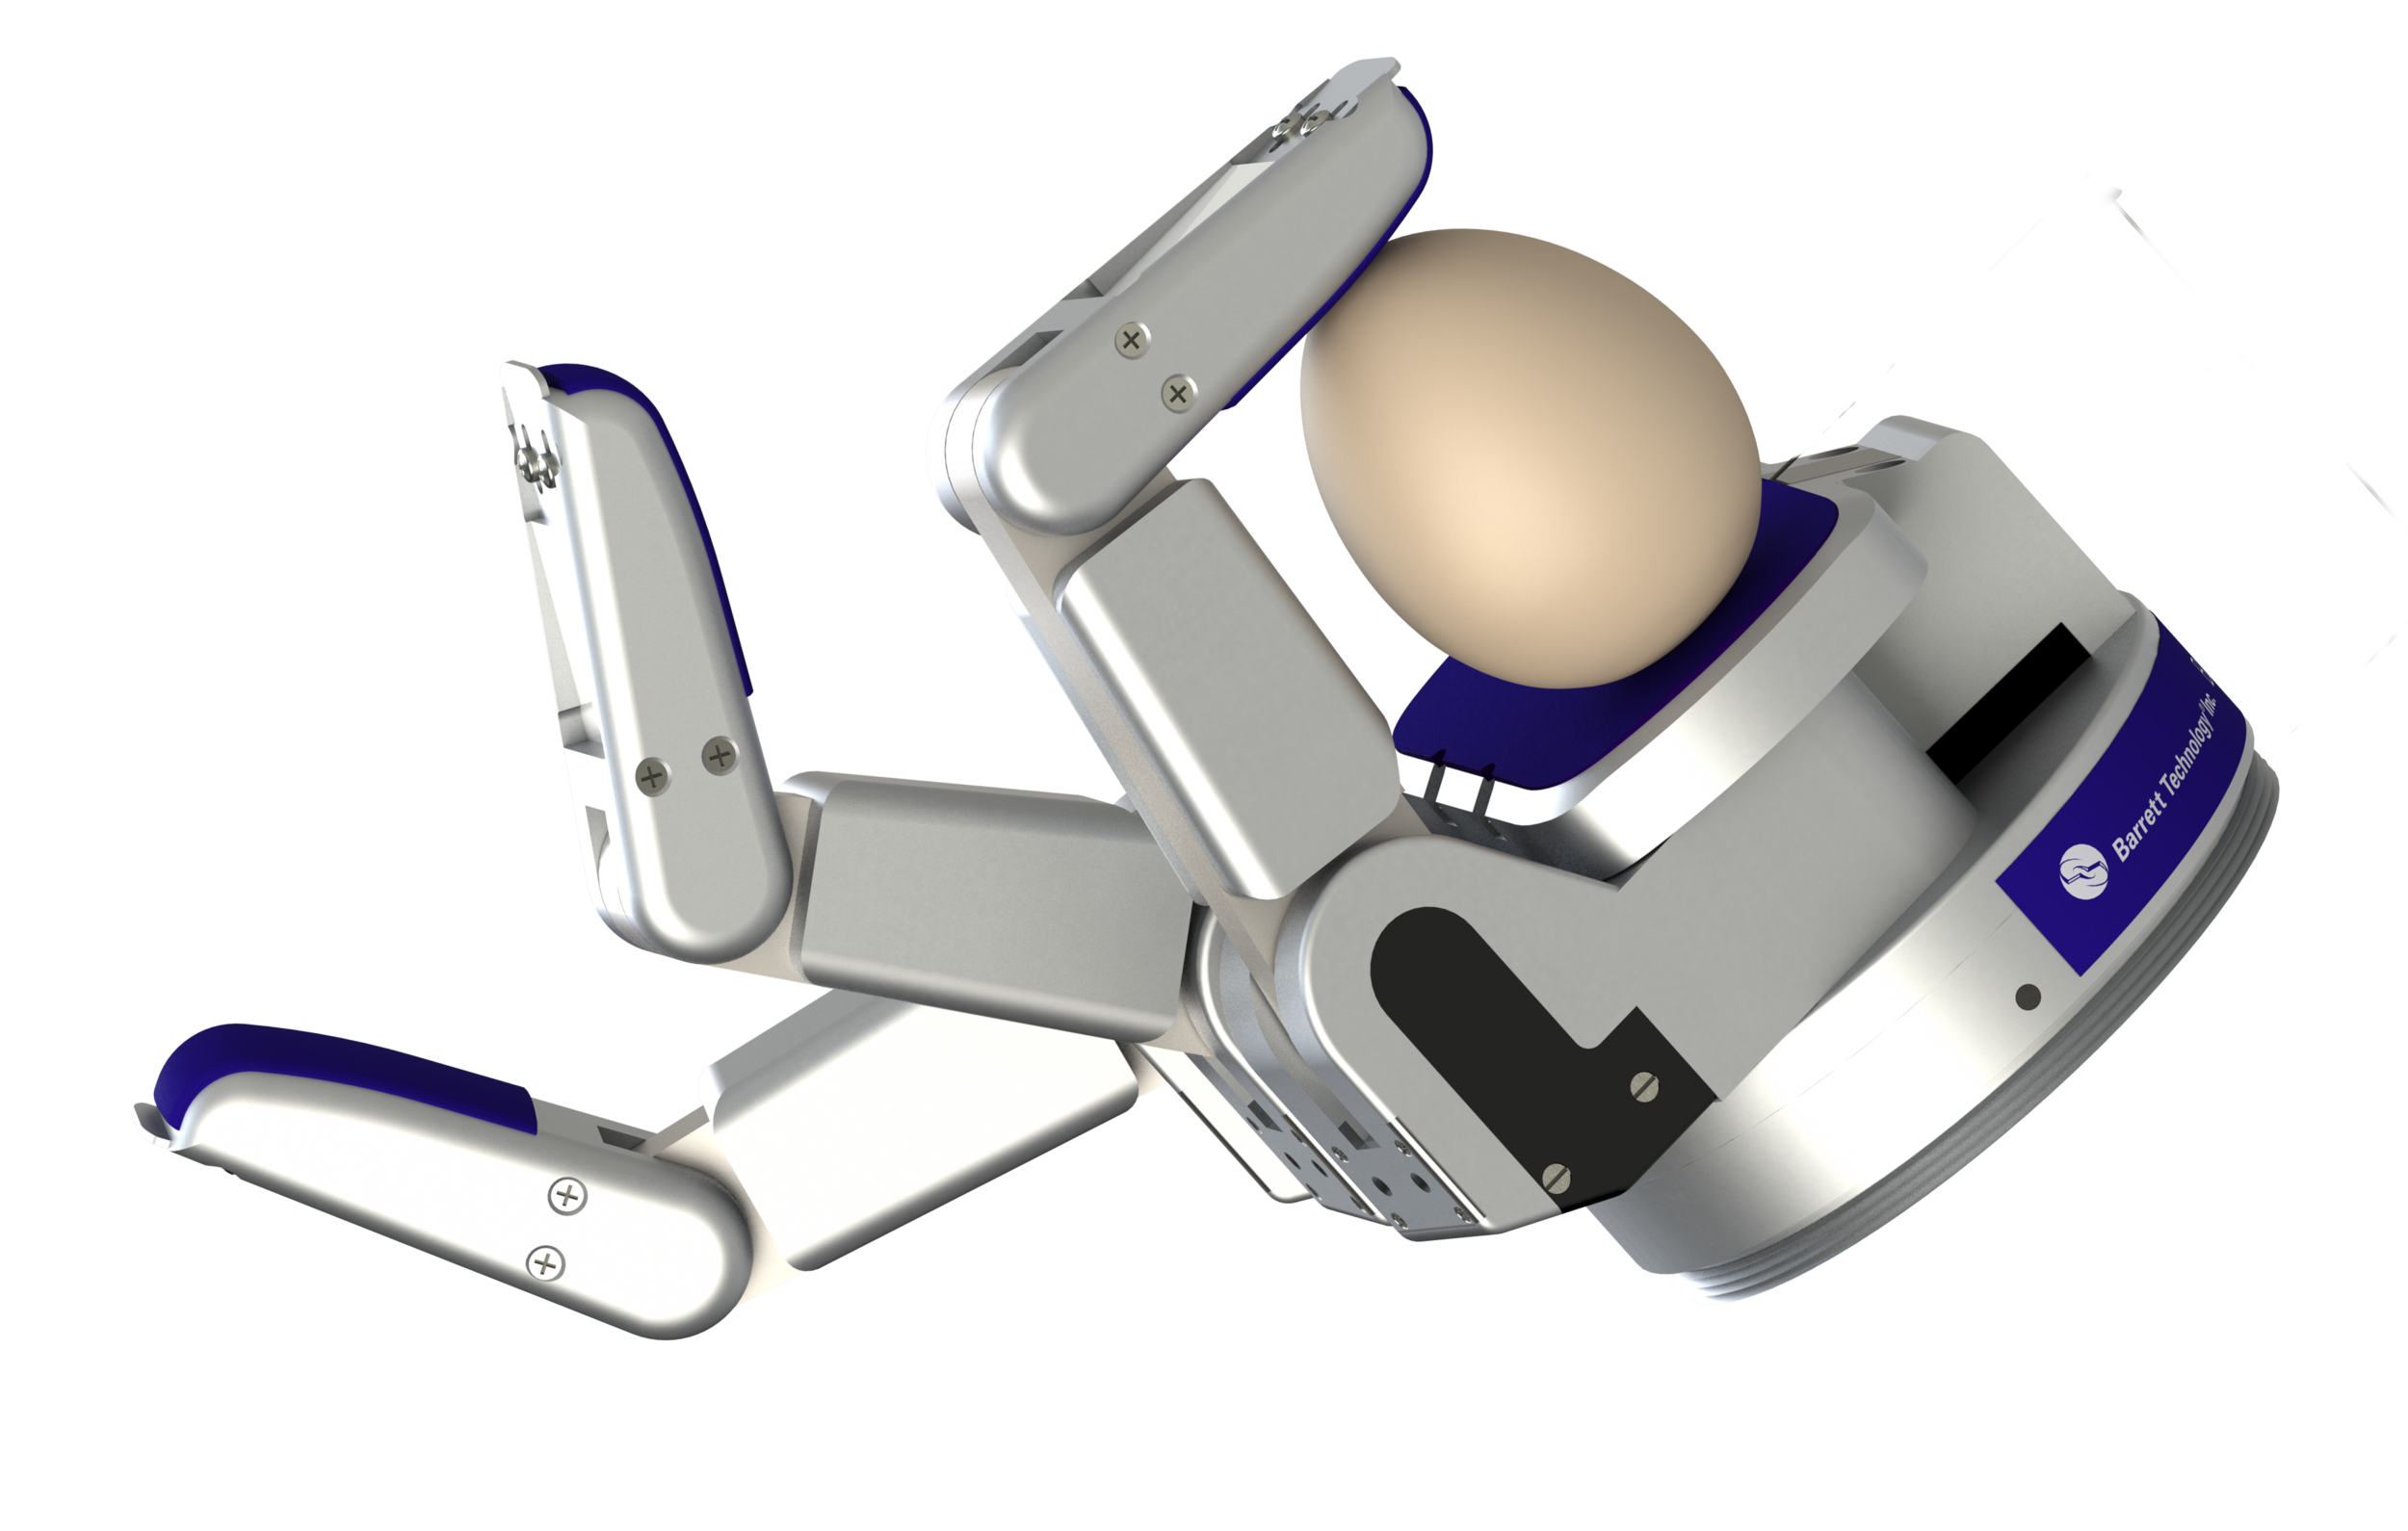
\includegraphics[scale=0.5]{barrett}
\end{figure}
\end{frame}

\begin{frame}{Robot usługowy Velma}
\begin{itemize}
	\item Dwa manipulatory LWR
	\item Chwytaki Barretta (sztuczna skóra, czujniki siły)
	\item Nadgarstkowe FTS
	\item Kinect
	\item Stereopara
	\item Komputer sterujący
\end{itemize}
\end{frame}

\begin{frame}{Oprogramowanie}
\begin{itemize}
	\item ROS
	\item Orocos
	\item Gazebo
	\item Linux RT
\end{itemize}
\end{frame}

\begin{frame}{Symulacja fizyki}
\begin{figure}
	\centering
	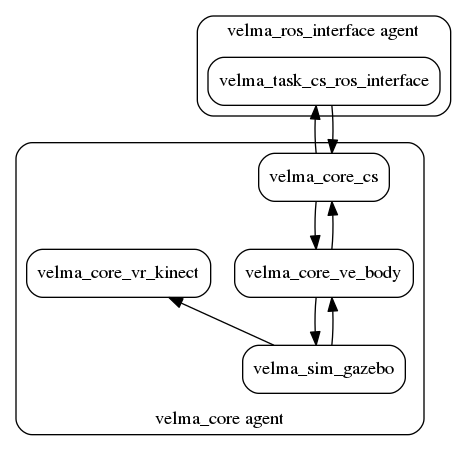
\includegraphics[scale=0.4]{simulation}
\end{figure}
\end{frame}

\begin{frame}{Rzeczywiste uruchomienie}
\begin{figure}
\centering
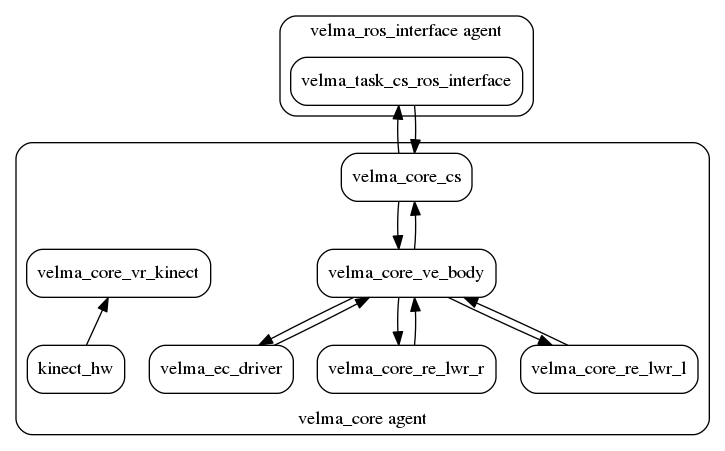
\includegraphics[scale=0.4]{real}
\end{figure}
\end{frame}

\section{Realizacja badań}
\begin{frame}{Koncepcja wykonania}
	\begin{itemize}
		\item Wdrożenie do systemu.
		\item Przegląd literatury.
		\item Zaprojektowanie modeli (może potrzebnych być kilka).
		\item Zaprojektowanie różnych algorytmów kompensacji grawitacji.
		\item Testy.
		\item Wybór zachowań zależnych od zaawansowania pozanania chwyconego obiektu.
	\end{itemize}
\end{frame}

\begin{frame}{Podejście naiwne}
\begin{itemize}
	\item Kompensacja tylko siłę grawitacji. 
	\item Używamy tradycyjnych regulatorów (PID, MPC, ...) z arbitralnie założonymi parametrami.
\end{itemize}
	
\end{frame}

\begin{frame}{Modele}
Najbardziej prawdopodobnym wyborem jest model bryły sztywnej.
\begin{itemize}
	\item Masa
	\item Środek ciężkości
	\item Parametry bezwładności
	\item Prędkość i przyspieszenie
	\item Informacja z systemu wizyjnego
\end{itemize}
\end{frame}

\begin{frame}{Roboczy model: Masa i środek ciężkości}
	Potrzebujemy dwóch różnych chwytów.
	\[ M_i = -M_{max}cos(\theta_m)\]
	\begin{figure}
		\centering
		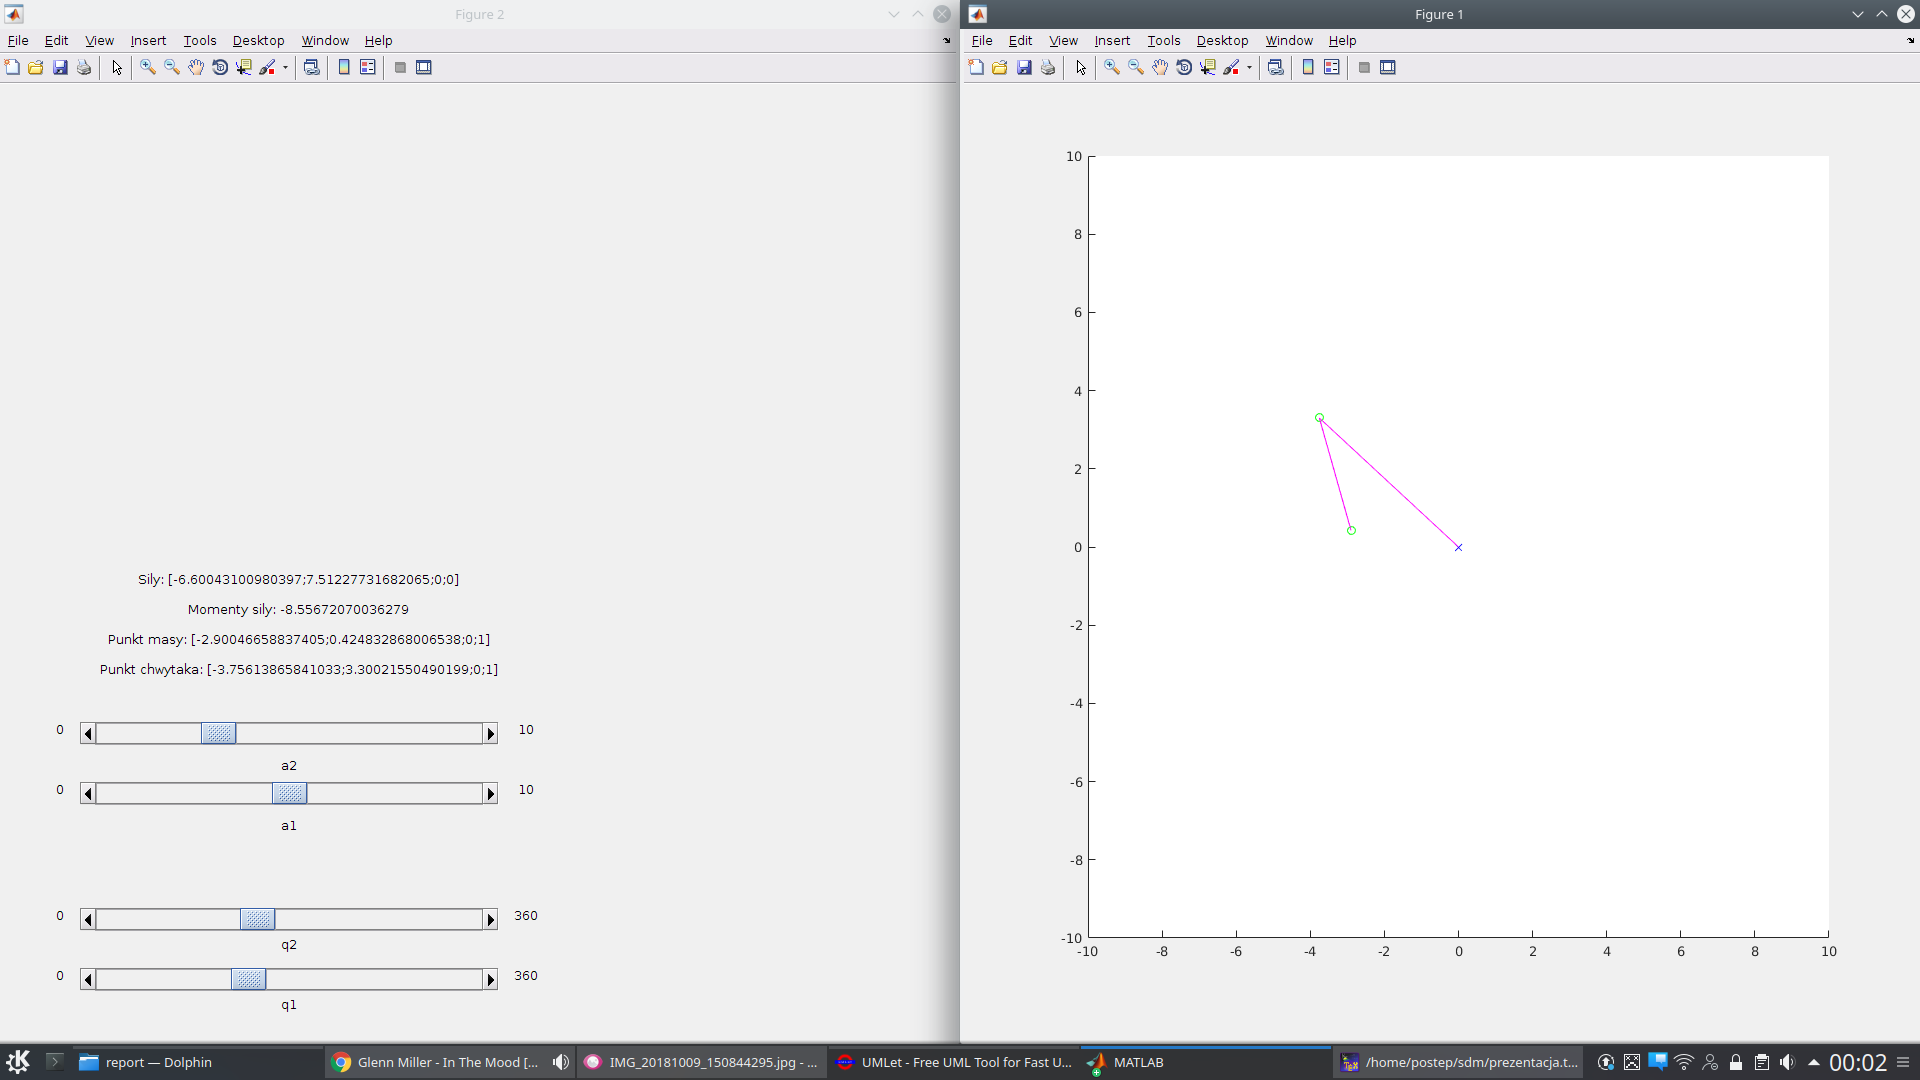
\includegraphics[scale=0.18]{matlab}
	\end{figure}
\end{frame}

\begin{frame}{Regulator adaptacyjny}
Należy zminimalizować uchyb pomiędzy pozycją osiąganą a zadaną.
\begin{figure}
	\centering
	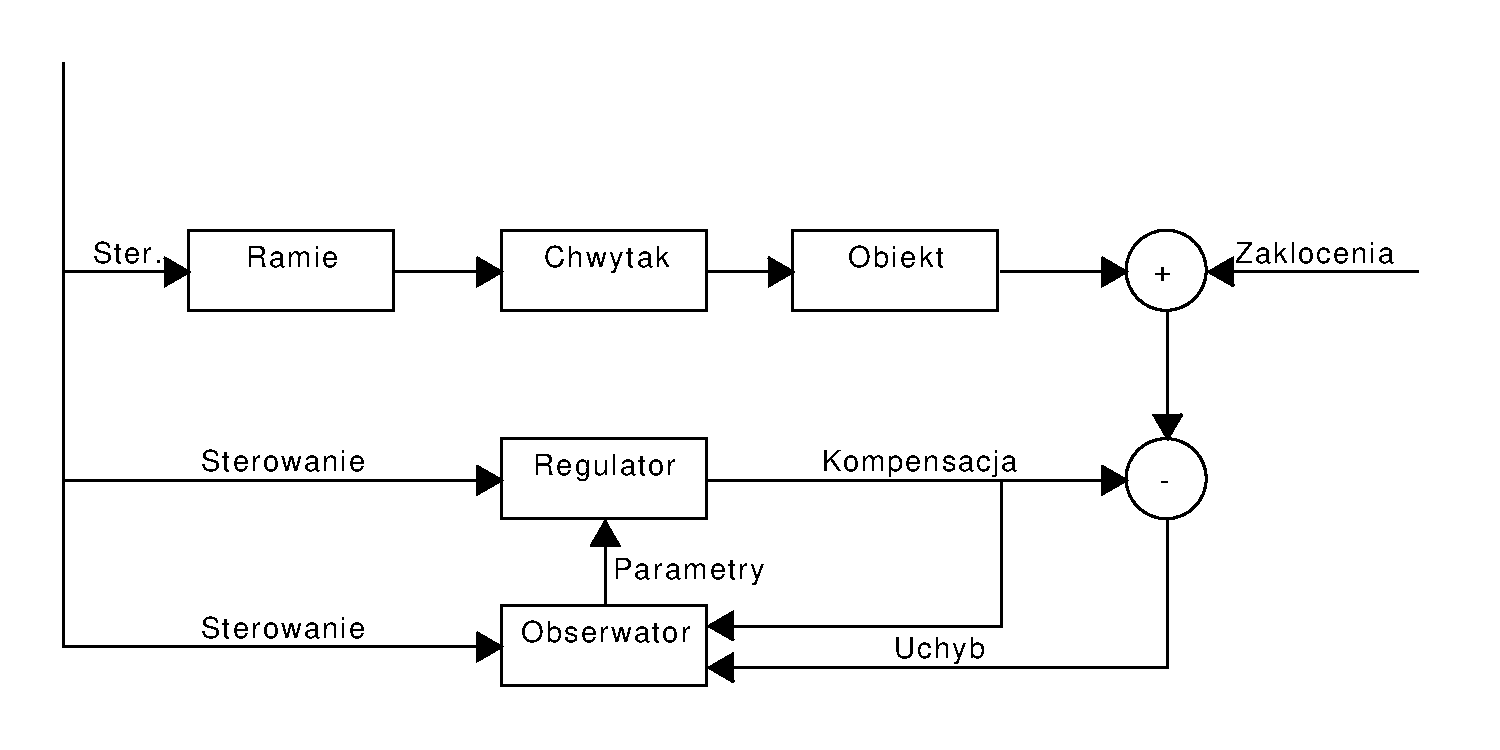
\includegraphics[scale=0.45]{reg}
\end{figure}

\end{frame}


%\begin{frame}[allowframebreaks]{Bibliografia}
%\bibliographystyle{plain}
%\bibliography{bibliography}
%\end{frame}
\section{Podsumowanie}
\begin{frame}{Ciekawy element badawczy}
Zastosowanie kompensacji siły grawitacji dla obiektu o nieznanym modelu.
\end{frame}

\begin{frame}{Bibliografia}
\begin{itemize}
	\item \url{https://robotyka.ia.pw.edu.pl}
	\item \url{http://osrobotics.org}
	\item Strony producentów.
\end{itemize}

\end{frame}
\begin{frame}{Dziękuję za uwagę}
\begin{figure}[h]
	\centering
	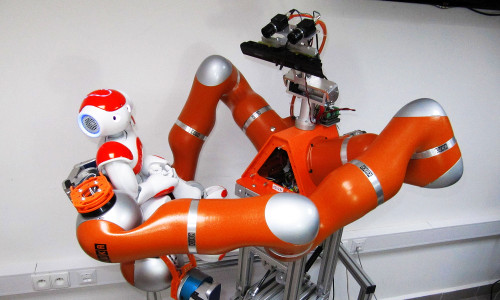
\includegraphics[scale=1.4]{velma3}
\end{figure}
\end{frame}
\end{document}